\chapter{Felhasználói dokumentáció}
\label{ch:user}

A program \texttt{Ubuntu 20.04} operációs rendszer alatt fut.
A futtatáshoz szükség van \texttt{Python 3.10.4}-re, valamint több könyvtárra,
ezeket a \texttt{requirements.txt} fájl tartalmazza, melyeket a
\texttt{pip} csomagkezelő segítségével könnyen feltelepíthetünk az alábbi
paranccsal: \texttt{pip install -r requirements.txt}

A programnak alapvetően két felhasználási módja van, egyrészt lehet saját
adatokkal tanítani a szegmentálást és a maszkolt C kód előállítását végző
modelleket, másrészt két, nagyszámú adaton előre betanított modellt használva
egy grafikus felület segítségével van lehetőség a lefordított C kódok
visszafejtésére.

\section{Tanítás}
Az Assembly kód szegmentálását és a maszkolt C kód előállítását két külön
neurális háló végzi, a felhasználónak ezek tanítására van lehetősge.
\subsection{Adatok}
A tanítási adatok egyszerű C fájlok, melyeket a \texttt{model/train/raw\_data}
mappában kell elhelyezni. Ezekből a nyers adatokból még ki kell nyerni
a tanításhoz szükséges információkat, ezt a \texttt{model/train/features.py}
script futtatásával tudjuk megtenni. Ez az előfeldogozott adatokat egy
\texttt{json} fájlba menti ki, ezt fogjuk a tanítások során majd használni

\subsection{Szegmentálás és fordítás tanítása}
A tanítási folyamatot a \texttt{model/train/segmentation\_train.py}, illetve
\texttt{model/train/translation\_train.py} program
futtatásával tudjuk elindítani. Ha nincs a gépünkön TPU vagy GPU, akkor először
egy figyelmeztető üzenetet ír ki a \texttt{Flax} könyvtár, hogy CPU-n fog futni
a program. Ezt követően a \texttt{Jax} könyvtár ír ki egy figyelmeztető
üzenetet, ez a könyvtár belső működésére vonatkozik, nyugodtan figyelmen kívül
hagyhatjuk.

\begin{figure}[H]
	\centering
	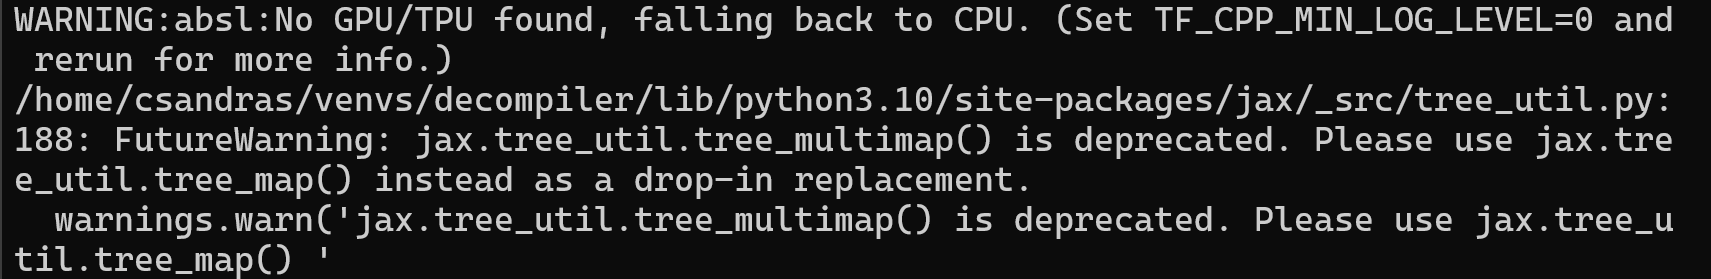
\includegraphics[width=1.0\textwidth]{images/warnings.png}
	\caption{A futtatás során kapott figyelmeztető üzenetek.}
	\label{fig:warnings}
\end{figure}

Ezután megjelenik egy folyamatjelző sáv, ami a felhasználó számára
jelzi, hogy az adott epoch-ban az adatok hányadrészét dolgozta fel eddig
a modell. Az epoch végén kiírja, hogy mennyi volt a hibája és a pontossága
a modellnek a tanító adatokon, majd a ugyanezt a tesztadatokra.

A program futása végén egy új ablakban megnyílik egy grafikon, ami külön
a tanító és teszt példákra szemlélteti, hogy a tanítás során mekkora volt
a modell hibája és pontossága. A felugró ablakot bezárva megjelenik egy üzenet,
hogy a betanított modell milyen néven mentődik el. A betanított
modellek a \texttt{model/train/runs} mappában érhetőek el. 

\begin{figure}[H]
	\centering
	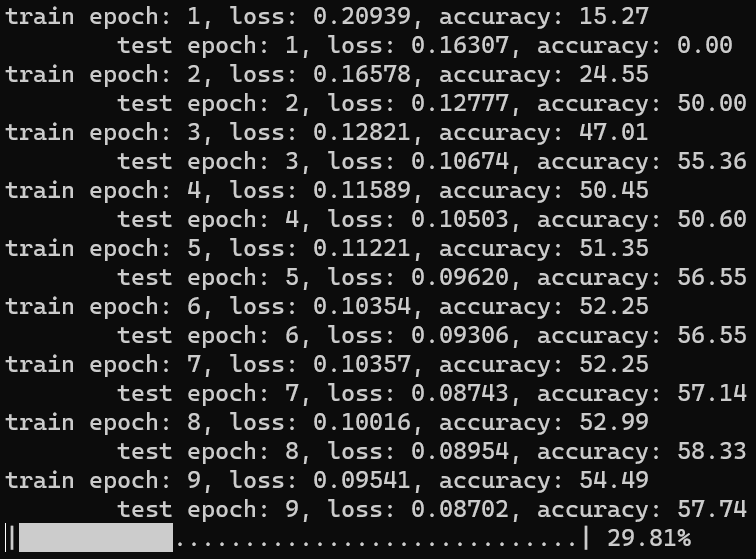
\includegraphics[width=0.8\textwidth]{images/translation_train.png}
	\caption[A fordítás tanítása]{A fordítás tanítása. A felhasználó számára egy folyamatjelző sáv
        mutatja, hogy az adott tanítási iterációban a tanítópéldák hány százalékát dolgozta fel
        eddig a modell. Ezen kívül látszik minden tanítási iterációra a modell hibája és pontossága
        a tanító-, valamint a tesztpéldákon.}
	\label{fig:train}
\end{figure}

\subsubsection{Szegmentálás konfigurálása}

A szegmentálás tanítása során használt paramétereket
a \texttt{model/train/segmentation\_train.yaml} fájlban lehet konfigurálni.
A felhasználó az alábbi beállításokat tudja módosítani:
\begin{itemize}
    \item \texttt{num\_epochs}: A tanulási iterációk száma, azt adja meg, hogy
        a modell összesen hányszor "látja" a teljes tanítóhalmazt. az
        alapértelmezett érték $10$.
    \item \texttt{optimizer}: A tanítási folyamat során milyen optimalizálót
        használjon a modell, az \texttt{optax}\cite{optax2020github} könyvtár
        alapértelmezett optimalizálói közül lehet választani. Az
        alapértelmezett érték \texttt{"adam"}\cite{adam}.
    \item \texttt{learning\_rate}: A tanulási ráta, azt szabályozza, hogy
    a gradiens módszer során milyen mértékben változtassa paramétereit
    a modell. Az alapértelmezett érték $0.003$.
    \item \texttt{hidden\_size}: Az \texttt{LSTM} által használt rejtett vektor
        mérete, az alapértelmezett érték $256$.
    \item \texttt{batch\_size}: A részmintaméret, azt lehet beállítani vele, hogy
        egy tanítási lépés során egyszerre hány adattal dolgozzon a modell. Az
        alapértelmezett érték $4$.
    \item \texttt{max\_len}: A bemenet, vagyis, hogy hány sor Assembly-ből áll
        a program, maximális hossza. Az alapértelmezett érték $90$.
    \item \texttt{embedding\_size}: A beágyazás után hány dimenziós vektort
        kapunk. Alapvetően a beágyazást egy előre betanított \texttt{Palmtree}\cite{palmtree}
        modell végzi, ami $128$ dimenziós vektorokkal dolgozik, így az
        alapértelmezett érték $128$, amit csak a \texttt{Palmtree} módosítása
        esetén változtassunk.
    \item \texttt{test\_ratio}: Az összes adat hányadrésze legyen a teszthalmaz
        (a maradék adat adja a tanítóhalmazt). Az alapértelmezett érték $0,2$.
\end{itemize}

\begin{figure}[H]
	\centering
    \captionsetup{singlelinecheck=off}
	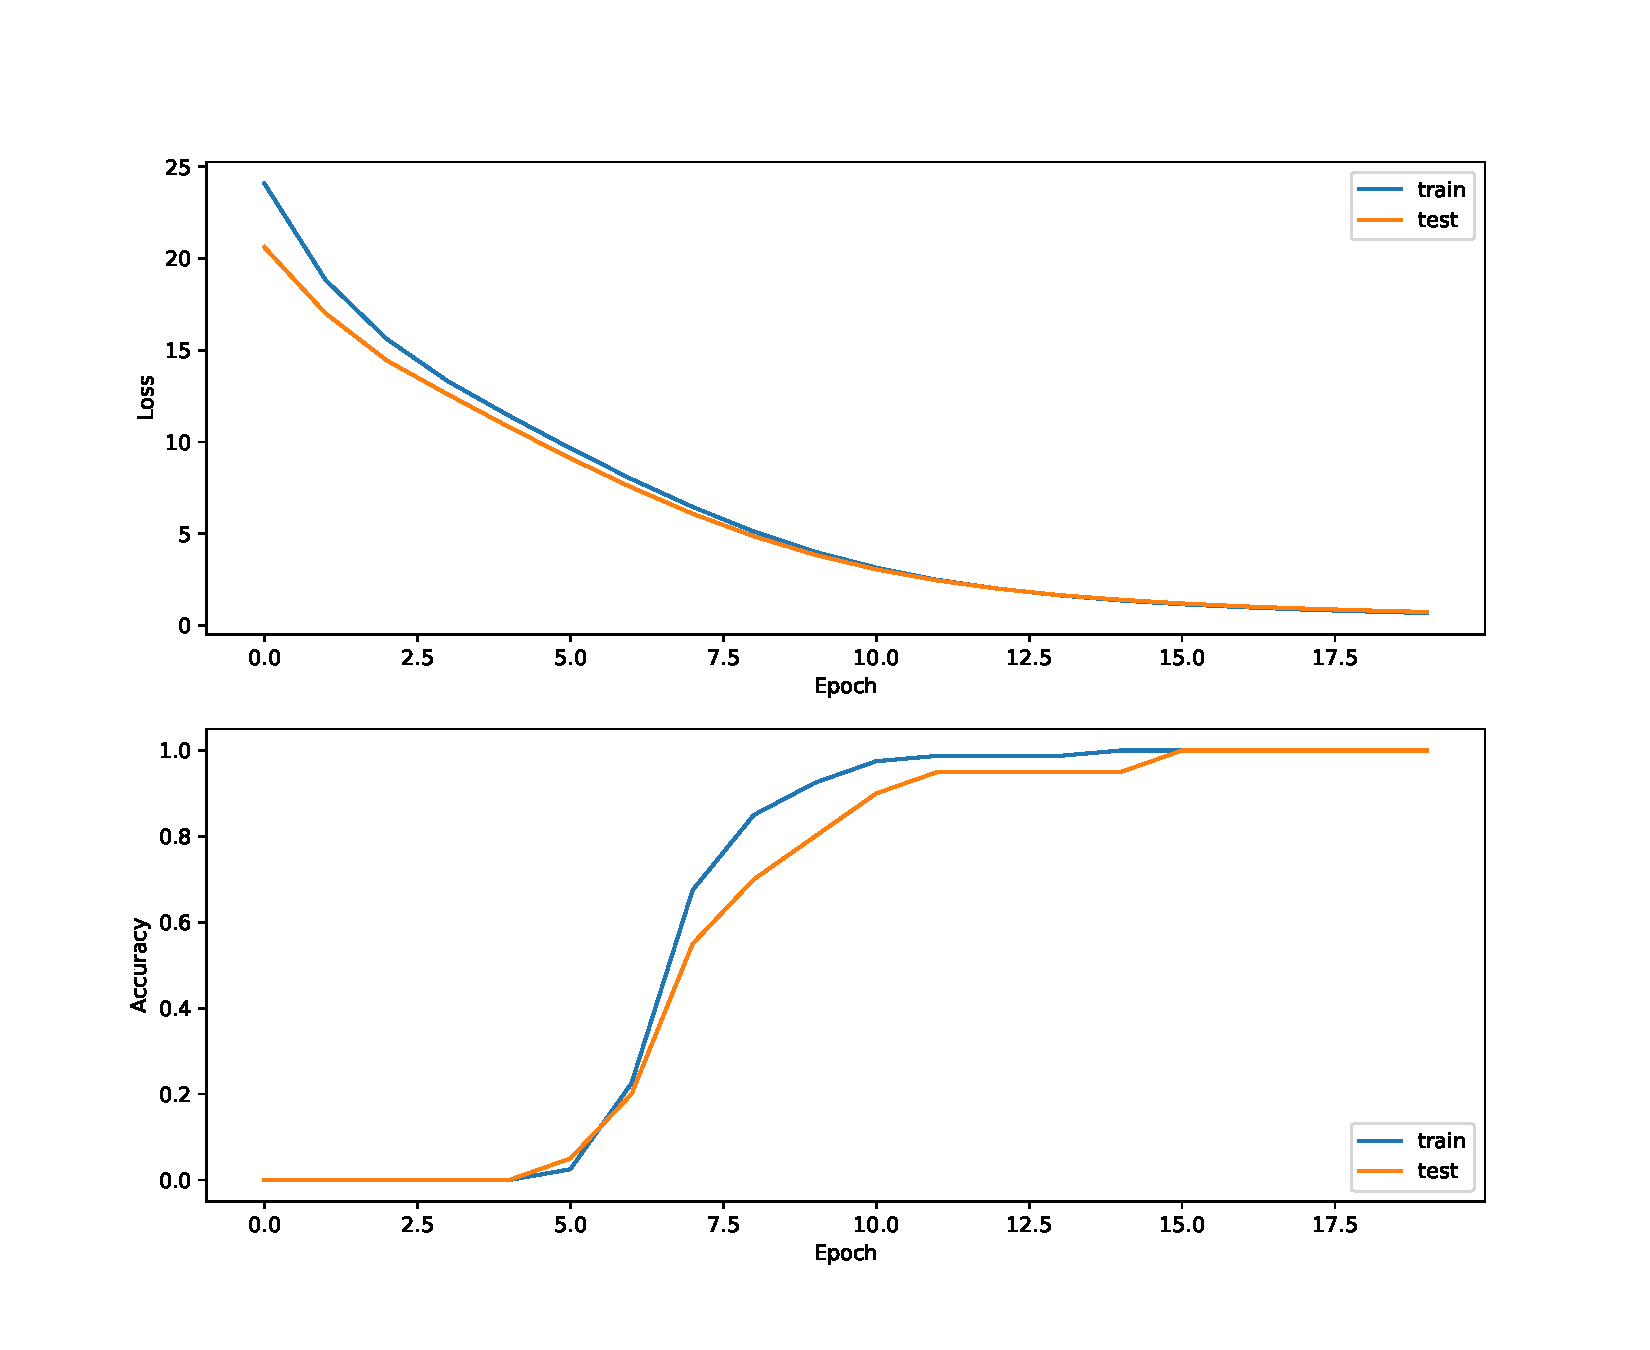
\includegraphics[width=1\textwidth]{images/segmentation_train.pdf}
	\caption[A hiba és a pontosság változása a szegmentálás tanítása során.]%
    {A hiba és a pontosság változása a tanító- és tesztpéldakon a szegmentálás tanítása során.\\
    A modell a következő paraméterekkel lett tanítva:
    \begin{itemize}
        \item \texttt{num\_epochs}: $20$
        \item \texttt{optimizer}: \texttt{"adam"}
        \item \texttt{learning\_rate}: $0.0003$
        \item \texttt{hidden\_size}: $128$
        \item \texttt{batch\_size}: $8$
        \item \texttt{max\_len}: $90$
        \item \texttt{embedding\_size}: $128$
        \item \texttt{test\_ratio}: $0.2$
    \end{itemize}}
	\label{fig:plot1}
\end{figure}

\subsubsection{Fordítás konfigurálása}

A fordítás tanítása során használt paramétereket
a \texttt{model/train/translation\_train.yaml} fájlban lehet konfigurálni.
A felhasználó az alábbi beállításokat tudja módosítani:
\begin{itemize}
    \item \texttt{num\_epochs}: Ld. szegmentálás konfigurálása.
    \item \texttt{optimizer}: Ld. szegmentálás konfigurálása.
    \item \texttt{learning\_rate}: Ld. szegmentálás konfigurálása.
    \item \texttt{hidden\_size}: Ld. szegmentálás konfigurálása.
    \item \texttt{batch\_size}: Ld. szegmentálás konfigurálása.
    \item \texttt{max\_input\_len}: A bemenet, vagyis, hogy hány sor
        Assembly-ből áll egy visszafordítandó blokk, maximális hossza. Az
        alapértelmezett érték $40$.
    \item \texttt{max\_output\_len}: A kimenet, vagyis, hogy hány token-ből
        állhat a visszafordítás során kapott maszkolt C kód, maximális hossza.
        Az alapértelmezett érték $40$.
    \item \texttt{test\_ratio}: Ld. szegmentálás konfigurálása.
\end{itemize}

\section{Betanított modell használata}
\subsection{Grafikus interfész}
A \texttt{main.py} programot futtatva egyrészt megjelennek a korábban írt
figyelmeztető üzenetek a konzolon, másrészt egy új ablakban a program grafikus
felülete. Itt a \texttt{Browse} gombra kattintva kiválaszthatjuk
a visszafejteni kívánt fájlt, majd ezt a \texttt{Submit} gombra kattintva
tudjuk betölteni. Ekkor a baloldali szövegdobozban megjelenik a kiválasztott futtatható
állományból kinyert Assembly kód.

\begin{figure}[H]
	\centering
	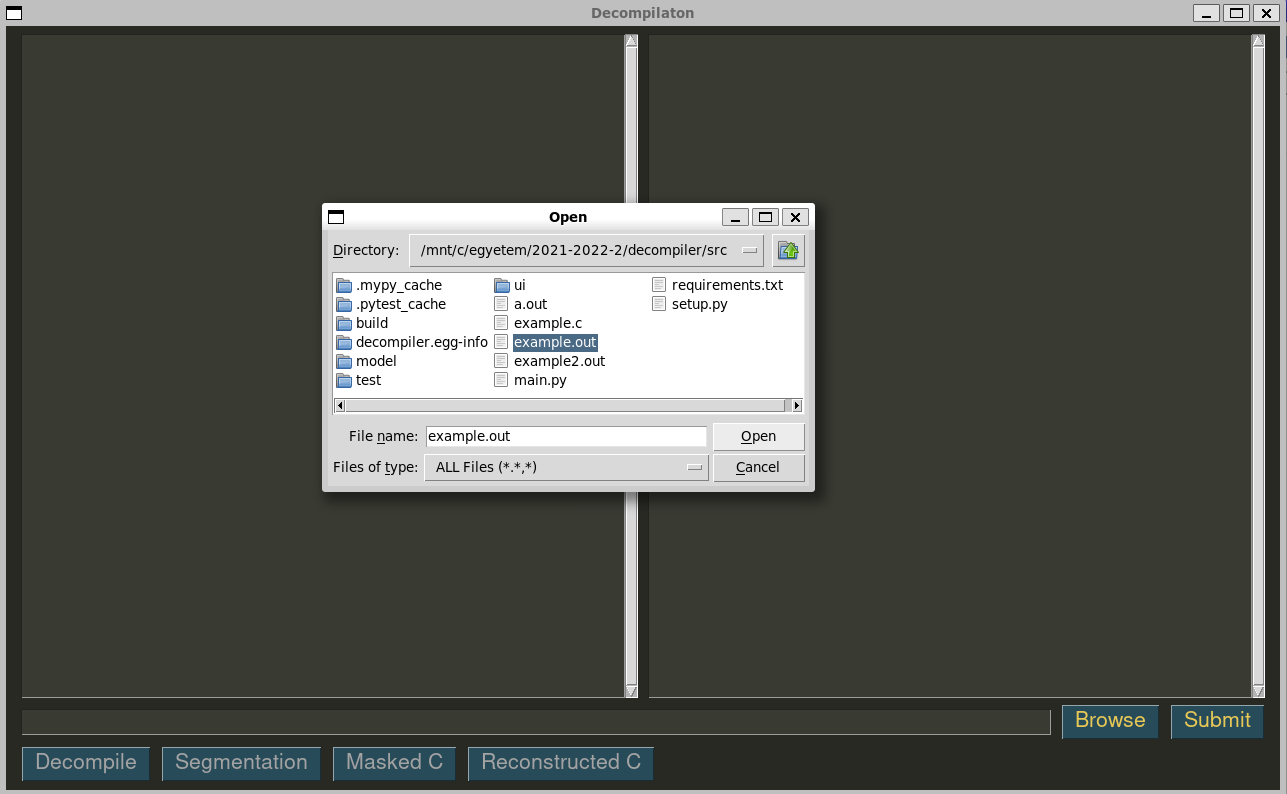
\includegraphics[width=1.0\textwidth]{images/file_browse.png}
	\caption{A visszafejtendő fájl betöltése a grafikus felületen.}
	\label{fig:file_browse}
\end{figure}

Ezután a \texttt{Decompile} gombra kattintva a jobboldali szövegdobozban megjelenik
a \texttt{Decompiling code, it may take a few seconds} felirat, majd
megkezdődik a kód visszafordítása, ami az eredeti C kód bonyolultságától
függően néhány másodperctől fél percig tart. A kódvisszafejtés végeztével
a szövegdobozban a következő szöveg jelenik meg: \texttt{Decompilaton done,
click on the buttons below to see the result.}

Ezután megnézhetjük, hogy
a bevezetésben leírt lépesek hogy zajlottak. a \texttt{Segmentation} gombra
kattintva a jobboldali szövegdobozban megjelenik a feldarabolt Assembly,
a blokkokat egy-egy üres sor választja el. A \texttt{Masked C} gombra kattintva
megjelenik az eredeti C kód "sablonja", itt még az összes változó helyén
a \texttt{VAR} token, a számliterálok helyén pedig a \texttt{NUM} token
szerepel. A \texttt{Reconstructed C} gombra kattintva pedig az iteratív
rekonstruálás során visszafejtett C kód jelenik meg a szövegdobozban, ami
szerkezetében megegyezik\footnote{A betanított modellek nem $100\%$
pontosságúak, így nem garantált, hogy mindig sikeres lesz a visszafordítás.} az
eredeti C kóddal.

\begin{figure}[H]
	\centering
	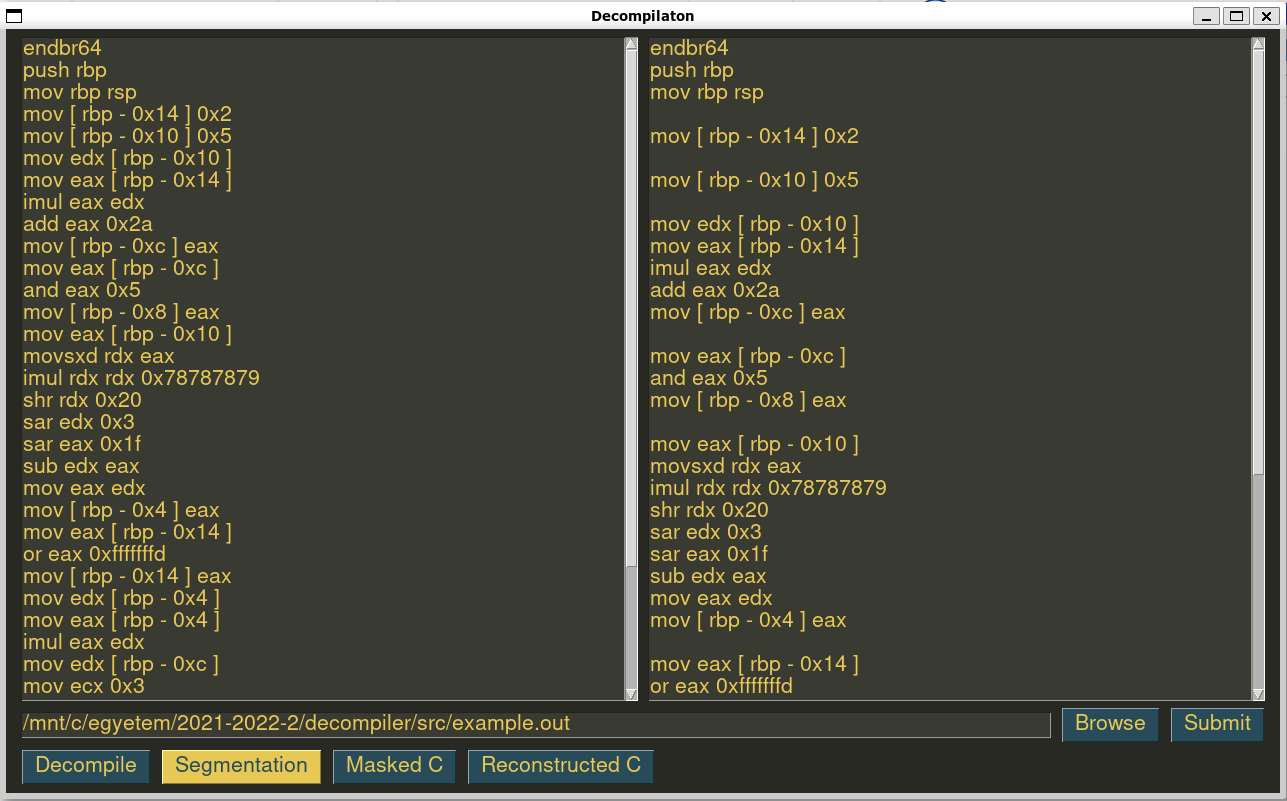
\includegraphics[width=1.0\textwidth]{images/segmentation.png}
	\caption{A szegmentálás megjelenítése a grafikus felületen.}
	\label{fig:segmentation}
\end{figure}

\begin{figure}[H]
	\centering
	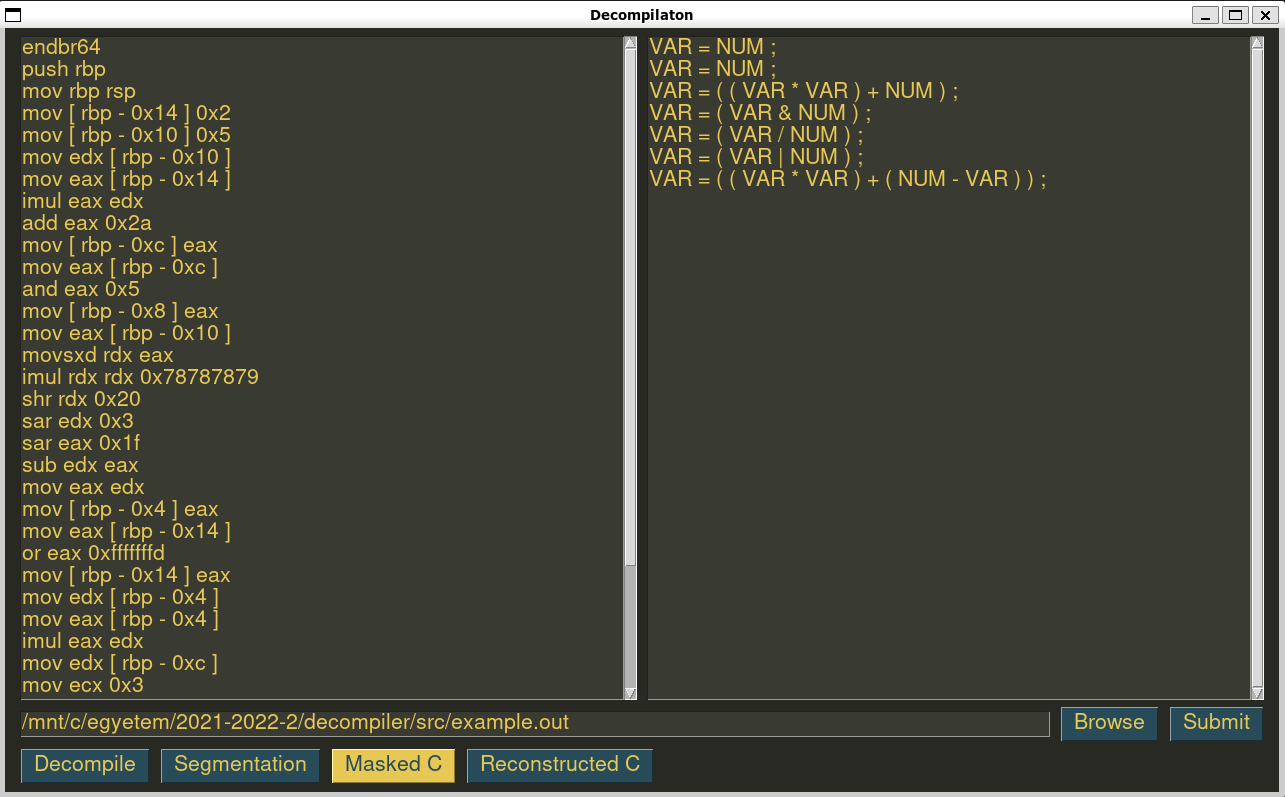
\includegraphics[width=1.0\textwidth]{images/masked_c.png}
	\caption{A maszkolt C kód megjelenítése a grafikus felületen.}
	\label{fig:masked_c}
\end{figure}

\begin{figure}[H]
	\centering
	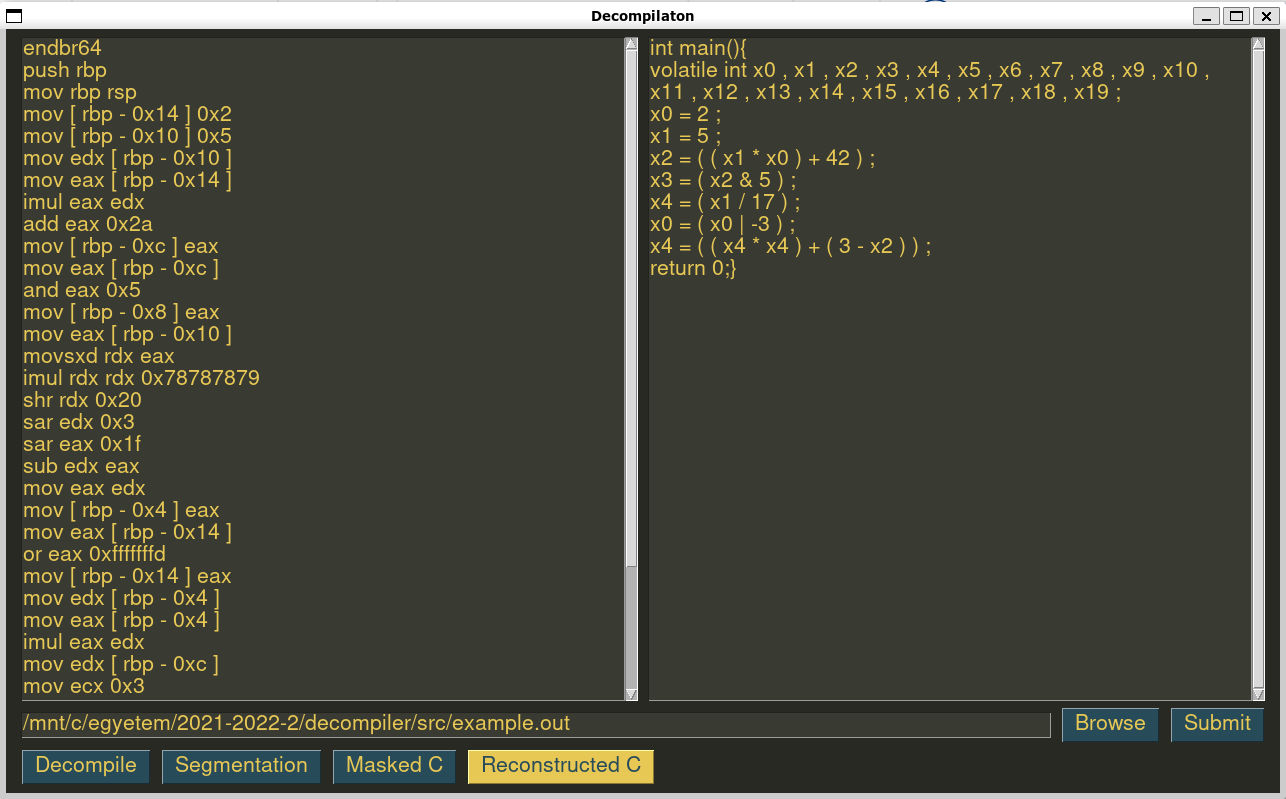
\includegraphics[width=1.0\textwidth]{images/reconstructed_c.png}
	\caption{A rekonstruált C kód megjelenítése a grafikus felületen.}
	\label{fig:reconstructed_c}
\end{figure}

\subsection{Konzolos interfész}
Ha a főprogramot a \texttt{\-\-gui=False} argumentummal futtatjuk, akkor egy
konzolos interfész segítségével is kipróbálhatjuk a program működését. Először
megjelennek a szokásos figyelmeztető üzenetek, majd a program bekéri
a visszafejtendő fájl nevét. Ide ha az \texttt{exit} parancsot írjuk, akkor
a program a \texttt{Closing program...} szöveget írja ki a képernyőre és
leáll a program futása. Ha nem létező fájlnevet adunk meg vagy nem megfelelő
formátumű a fájl, akkor a program egy
\texttt{File \textit{fájlnév} not found} hibaüzenetet ír ki, majd leáll a program.
Ha létezik a fájl és megfelelő formátumú,
akkor a program rögtön elkezdi a visszafordítást, ez általában egy pár
másodperces folyamat, bonyolultabb programok esetén kicsivel több.

\begin{figure}[H]
	\centering
	\subcaptionbox{A modell bementét képező Assembly kód.}{
		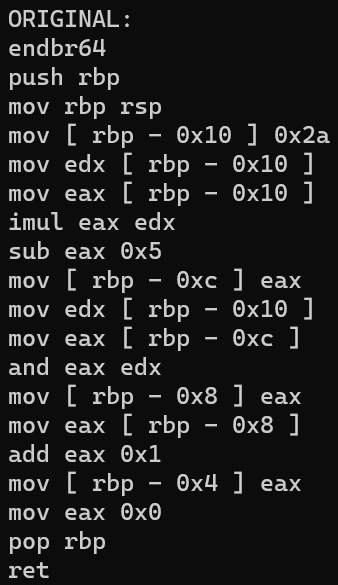
\includegraphics[width=0.25\linewidth]{images/original_cli.png}}
	\hspace{5pt}
	\subcaptionbox{A szegmentált Assembly kód.}{
		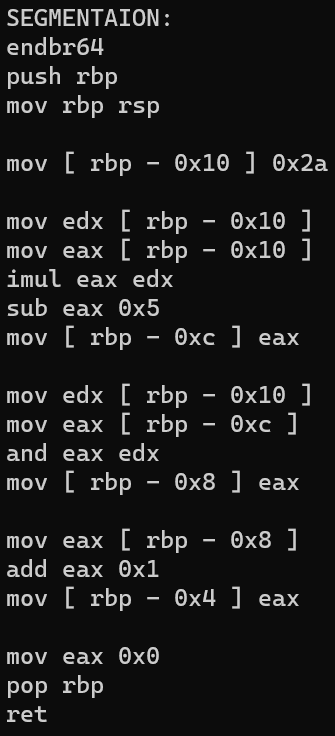
\includegraphics[width=0.25\linewidth]{images/segmentation_cli.png}}
	\hspace{5pt}
	\subcaptionbox{A maszkolt C kód.}{
		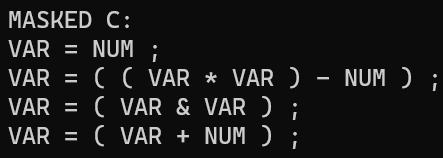
\includegraphics[width=0.4\linewidth]{images/masked_c_cli.png}}
	\hspace{5pt}
	\subcaptionbox{A rekonstruált C kód.}{
		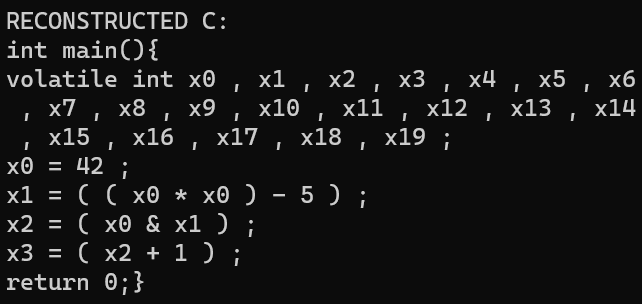
\includegraphics[width=0.6\linewidth]{images/reconstructed_c_cli.png}}
	\caption{A kódvisszafejtés lépései a konzolos interfészen.}
	\label{fig:cli}
\end{figure}

\subsection{A modell konfigurálása}
A modell különböző paramétereit a \texttt{model/model\_config.yaml} fájlban
lehet konfigurálni. A felhasználó az alábbi beállításokat tudja módosítani:
\begin{itemize}
    \item \texttt{segmentation/model\_path}: A szegmentálás során használt
        modell relatív elérési útvonala. Az alapértelmezett érték
        \texttt{"flax\_models/segmentation.params"}, ez egy előre, sok adaton
        betanított modell. A felhasználónak lehetősége van a tanítási folyamat
        során elmentett modellek betöltésére is, ekkor annak a relatív elérési
        útvonalát kell megadni.
    \item \texttt{segmentation/hidden\_size}: Ld. szegmentálás konfigurálása.
    \item \texttt{segmentation/max\_len}: Ld. szegmentálás konfigurálása.
    \item \texttt{translation/model\_path}: A fordítás során használt modell
        relatív elérési útvonala. Az alapértelmezett érték
        \texttt{"flax\_models/translation.params"}, ez egy előre, sok adaton
        betanított modell. A szegmentáláshoz hasonlóan itt is van lehetőség
        a felhasználó által betanított modellek betöltésére az útvonal
        módosításával.
    \item \texttt{translation/vocab\_path}: Ide egy json formátumú fájl elérési
        útvonalát kell megadni, ami egy szótárat tartalmaz, melyben szerepel,
        hogy a lehetséges kimeneti tokeneket milyen számra képezzük. Az
        alapértelmezett érték \texttt{"flax\_models/vocab.json"}.
    \item \texttt{hidden\_size}: Ld. szegmentálás konfigurálása.
    \item \texttt{max\_input\_len}: Ld. fordítás konfigurálása.
    \item \texttt{max\_output\_len}: Ld. fordítás konfigurálása.
\end{itemize}

